\documentclass{article}
% translate with >> pdflatex -shell-escape <file>

% This file is used as unit test for pgfplots, copyright by Christian Feuersaenger.
% 
% See
%   http://pgfplots.sourceforge.net/pgfplots.pdf
% for pgfplots.
%
% Any required input files (for <plot table> or <plot file> or the table package) can be downloaded
% at
% http://www.ctan.org/tex-archive/graphics/pgf/contrib/pgfplots/doc/latex/
% and
% http://www.ctan.org/tex-archive/graphics/pgf/contrib/pgfplots/doc/latex/plotdata/

\usepackage{pgfplots}
\pgfplotsset{compat=newest}

\pagestyle{empty}

\begin{document}
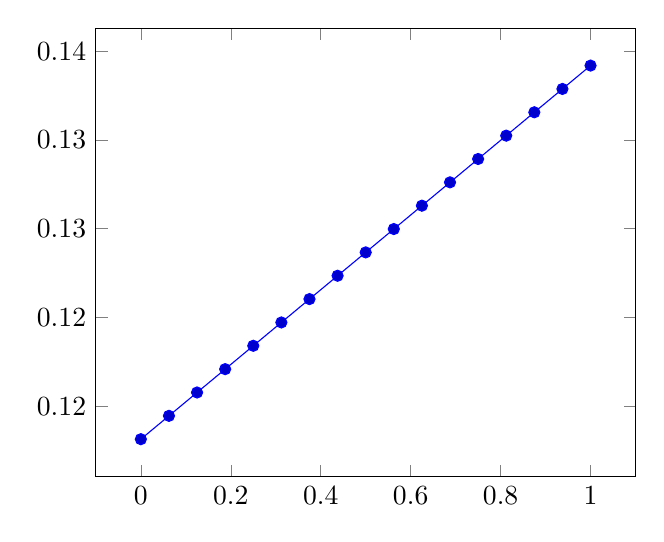
\begin{tikzpicture}%
\begin{axis}
\addplot plot coordinates {
	(0.000000,	0.113142)
	(0.062500,	0.114457)
	(0.125000,	0.115773)
	(0.187500,	0.117088)
	(0.250000,	0.118404)
	(0.312500,	0.119719)
	(0.375000,	0.121035)
	(0.437500,	0.122350)
	(0.500000,	0.123666)
	(0.562500,	0.124981)
	(0.625000,	0.126297)
	(0.687500,	0.127612)
	(0.750000,	0.128928)
	(0.812500,	0.130243)
	(0.875000,	0.131559)
	(0.937500,	0.132874)
	(1.000000,	0.134190)
};
\end{axis}
\end{tikzpicture}
\end{document}
